\documentclass[border=12pt]{standalone}
\usepackage{tikz}
\usetikzlibrary{shapes.geometric, arrows.meta, positioning, calc, fit, backgrounds}
\usepackage{fontspec}
\usepackage{amsmath,amssymb}
\setmainfont{DejaVu Sans}

\begin{document}
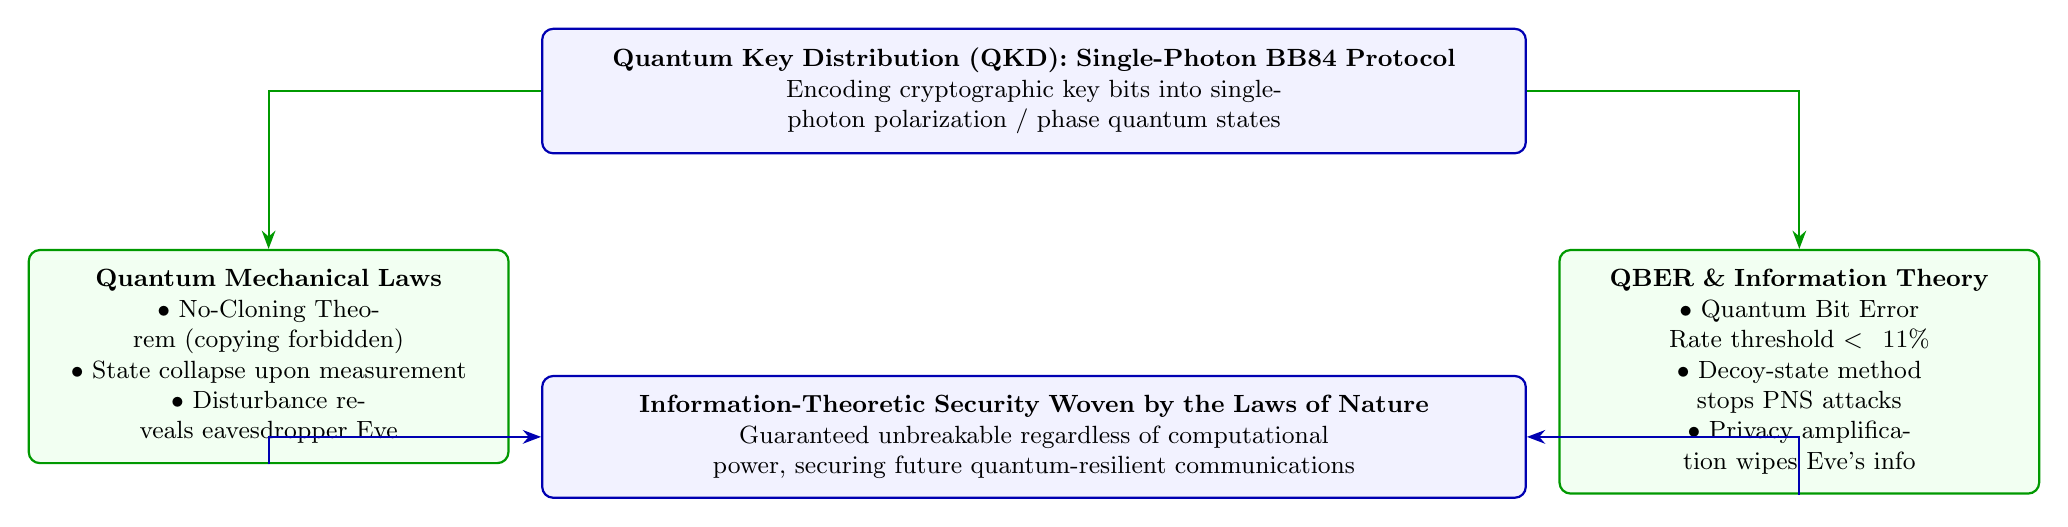
\begin{tikzpicture}[
    font=\small,
    >=Stealth,
    node distance=1.2cm,
    block/.style={rectangle, draw=blue!70!black, fill=blue!5, rounded corners=4pt, thick, align=center, inner sep=7pt},
    alertblock/.style={rectangle, draw=red!70!black, fill=red!5, rounded corners=4pt, thick, align=center, inner sep=7pt},
    greenblock/.style={rectangle, draw=green!60!black, fill=green!5, rounded corners=4pt, thick, align=center, inner sep=7pt},
    amberblock/.style={rectangle, draw=orange!80!black, fill=orange!5, rounded corners=4pt, thick, align=center, inner sep=7pt}
]

\node[block, text width=12cm] (top) {\textbf{Quantum Key Distribution (QKD): Single-Photon BB84 Protocol}\\Encoding cryptographic key bits into single-photon polarization / phase quantum states};

\node[greenblock, below left=1.2cm and 0.4cm of top, text width=5.6cm] (physics) {\textbf{Quantum Mechanical Laws}\\$\bullet$ No-Cloning Theorem (copying forbidden)\\$\bullet$ State collapse upon measurement\\$\bullet$ Disturbance reveals eavesdropper Eve};

\node[greenblock, below right=1.2cm and 0.4cm of top, text width=5.6cm] (qber) {\textbf{QBER \& Information Theory}\\$\bullet$ Quantum Bit Error Rate threshold $< 11\%$\\$\bullet$ Decoy-state method stops PNS attacks\\$\bullet$ Privacy amplification wipes Eve's info};

\node[block, below=2.8cm of top, text width=12cm] (bottom) {\textbf{Information-Theoretic Security Woven by the Laws of Nature}\\Guaranteed unbreakable regardless of computational power, securing future quantum-resilient communications};

\draw[->, thick, green!60!black] (top) -| (physics);
\draw[->, thick, green!60!black] (top) -| (qber);
\draw[->, thick, blue!70!black] (physics) |- (bottom);
\draw[->, thick, blue!70!black] (qber) |- (bottom);

\end{tikzpicture}
\end{document}
